\chapter{Experimental Results}
\label{chap:Results} 

\section{Reconstruction}

\subsection{Quantitative Results}

\subsubsection{GMM}

All proposed methods are able to increase the main network's accuracy and
validation accuracy (\cref{tab:gmm_results}) 
over the baseline results after the distortion has been applied (\cref{tab:gmm_baseline}).
Also, the accuracy reported by the verification network is increased.
It is interesting to note that even though nearly all methods 
are able to decrease the the cross-entropy\footnote{
For a larger number of samples, the data set cross-entropy is reported as infinity.
This is due to floating point precision errors that arise even with overflow measures in place.},
the l2-error after reconstruction is always increased.

However, it is important to remember that the loss function used in the optimization process
is a composite loss from the proposed loss between the statistics
and the original cross-entropy loss used in the optimization of the neural network.
\[
    r_{stats} \loss(\set A, \set B) + r_{crit}\loss_{crit}(\set B, y_{\set B})
\]
Since, by itself, the original criterion loss alone already performs quite well, 
it can be said that the proposed losses act as a kind of regularization 
by incorporating more knowledge about the target data distribution 
that prevent overfitting
of the target data set.

A comparison of the results for the case $r_{crit}=0$ can be found in \cref{tab:gmm_results_raw}.
In this scenario, two methods, namely NN CC and RP CC seem to give 
better generalization scores 
(validation and verification accuracy) than when the original cross-entropy loss 
$\loss_\text{crit}$ is included.
But it is hard to explain the lower cross-entropy when leaving out 
$\loss_\text{crit}$, which is specifically designed to minimize \cref{eqn:cross_entropy}, 
the cross-entropy.
Nevertheless, it is important to note that scores can fluctuate a fair amount and more 
experiment runs are necessary to give a clearer picture.
These results also show that, unsupervised, i.e. without class information, 
none of the presented methods is able to yield good results.


\begin{table}[!htbp]
\centering
\footnotesize
\pgfplotstabletypeset[
baseline,
gmm,
]{figures/reconstruction_GMM_baseline.csv}
\caption{GMM baseline scores}
\label{tab:gmm_baseline}
\end{table}

\begin{table}[!htbp]
\centering
\footnotesize
\pgfplotstabletypeset[
results,
gmm,
every row 6 column 1/.style={highlight},
every row 8 column 1/.style={highlight},
every row 10 column 1/.style={highlight},
every row 11 column 1/.style={highlight},
every row 7 column 2/.style={highlight},
every row 4 column 3/.style={highlight},
every row 8 column 4/.style={highlight},
every row 8 column 5/.style={highlight},
]{figures/reconstruction_GMM_results.csv}
\caption{Metrics on reconstruction results after 100 optimization epochs on GMM data set}
\label{tab:gmm_results}
\end{table}

\begin{table}[!htbp]
\centering
\footnotesize
\pgfplotstabletypeset[
results,
gmm,
every row 1 column 1/.style={highlight},
every row 7 column 2/.style={highlight},
every row 7 column 3/.style={highlight},
every row 4 column 4/.style={highlight},
every row 7 column 5/.style={highlight},
]{figures/reconstruction_GMM_results_raw.csv}
\caption{Metrics on reconstruction results after 100 optimization epochs for $r_\text{crit}=0$ on GMM data set. Non-CC methods work entirely without label information and can be said to operate in an unsupervised setting.}
\label{tab:gmm_results_raw}
\end{table}


When reviewing the trajectories of the scores (as seen in \cref{fig:metrics_GMM_l2_increase}), 
many of the methods show that soon after the loss passes a reference value 
- the same loss calculated on a batch of unperturbed data - 
the l2-error is seen to increase. 


\begin{figure}[!htbp]
    \centering
    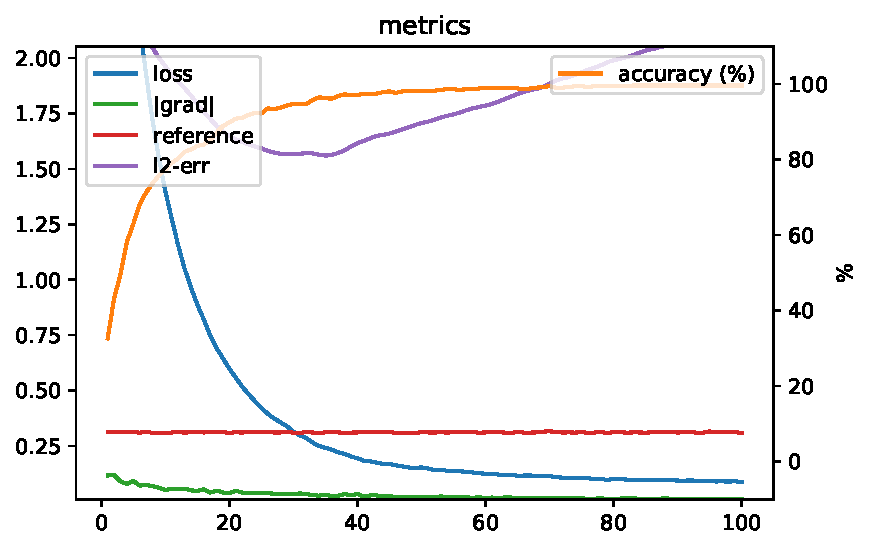
\includegraphics[width=0.7\textwidth]{figures/reconstruction_GMM_NN_ALL_metrics.pdf}
    \caption{Plot of optimization metrics of method NN ALL \\on the GMM data set}
    \label{fig:metrics_GMM_l2_increase}
\end{figure}

\subsubsection{MNIST}


The distortion factor ($\kappa = 0.2$) on the MNIST data set is chosen to be fairly strong.
After the distortion is applied, the overall accuracies drop from 97-99\% (\cref{tab:mnist_baseline})
to near random guesses $\frac 1 C \approx 10\%$ (\cref{tab:mnist_results}).
% The results for the reconstruction task for all methods on the MNIST data set is depicted in .
The criterion (CRITERION) alone gives good results when evaluated by the main network, 
yet fails when tested on a second network.
This puts into question the validity of the neural network's classification process.
It is possible for the neural network to learn non-robust features (\cite{ilyas2019adversarial})
that, 
are able to correctly identify a large part of the data set, 
yet don't correspond to features we as humans might make out.
This problem has been studied by \cite{damour2020underspecification} 
and is termed as \textit{underspecification}.

The hardly improved verification score of NN, where additionally the second-to-last layer is 
incorporated, seems to confirm
the network's bias in the optimization procedure. 
An improvement in generalization can be seen only after taking 
all layers of the neural network (NN ALL) into account.
The randomly initialized neural network (RANDOM NN) does not add any significant improvement; 
it is not able to capture much important information about the data set.
Random projections (RP) is able to add an additional amount of regularization that is seen in the generalization scores.
Combining the methods (COMBINED) seems to merit overall good scores which can be verified in image quality.


\begin{table}[!htbp]
\centering
\footnotesize
\pgfplotstabletypeset[
results,
images,
display columns/0/.style={column name=\textbf{baseline}, column type=l, string type},
]{figures/reconstruction_MNIST_baseline.csv}
\caption{MNIST baseline scores}
\label{tab:mnist_baseline}
\end{table}

\begin{table}[!htbp]
\centering
\footnotesize
\pgfplotstabletypeset[
results,
images,
every row 11 column 1/.style={highlight},
every row 11 column 2/.style={highlight},
every row 11 column 3/.style={highlight},
every row 11 column 4/.style={highlight},
every row 5 column 5/.style={highlight},
every row 6 column 6/.style={highlight},
]{figures/reconstruction_MNIST_results.csv}
\caption{Metrics on reconstruction results after 100 optimization epochs on MNIST data set}
\label{tab:mnist_results}
\end{table}


Here it is noted, that the l2-error and the PSNR-score 
drop after the reconstruction task is performed.
As the qualitative results shown in \cref{AppendixResults} suggest otherwise,
this substantiates the concern that these scores might not be indicative of image quality.
The SSIM-score proves to be more robust in this regard, subjectively seen in the reconstructed images.



\subsubsection{CIFAR10}

The CIFAR10 data set is regarded as more complex than the previous two.
The depicted objects have greatly varying backgrounds and are shown from numerous different angles.
The feature representations are ideally able to represent invariant properties and to 
filter out the background noise.
The network for this data set is of a deeper (34 layers) architecture, and the
the learned feature representations seem to be more robust 
as the found reconstruction is validated by the verification network.

Random projections do not perform well on this task;
their design is too simple to be able to capture the complexities of the data set.
Since the randomly initialized network (RANDOM NN), 
also performs poorly,
it can be said that a good feature representation is necessary for this task.

\begin{table}[!htbp]
\centering
\footnotesize
\pgfplotstabletypeset[
baseline,
images,
]{figures/reconstruction_CIFAR10_baseline.csv}
\caption{CIFAR10 baseline scores}
\label{tab:cifar10baseline}
\end{table}

\begin{table}[!htbp]
\centering
\footnotesize
\pgfplotstabletypeset[
results,
images,
every row 2 column 1/.style={highlight},
every row 4 column 1/.style={highlight},
every row 3 column 2/.style={highlight},
every row 4 column 3/.style={highlight},
every row 3 column 4/.style={highlight},
every row 3 column 5/.style={highlight},
every row 3 column 6/.style={highlight},
]{figures/reconstruction_CIFAR10_results.csv}
\caption{Metrics on reconstruction results after 100 optimization epochs for CIFAR10}
\label{tab:cifar10results}
\end{table}





Of the methods using neural networks, NN ALL has overall the best performance.
This is confirmed by visual inspection in \cref{AppendixResults}.
By using the class-conditional version (NN ALL CC), one would expect better results.
However, this is not immediately seen in \cref{tab:cifar10results} and the images appear qualitatively worse. 
A reason why could be that the network is already complex enough to "split" the signal into distinct enough activations so that adding
a class-conditional formulation does not add more context.
It might even be a hindrance, because of the high variance in image statistics
from one image to another due to background "noise".
Since the class-conditional formulation groups inputs according to their respective classes, 
it is possible that, due to random sampling, one iteration contains 
few samples of one class. Alternatively, one grouped batch could
display unusual statistics (e.g. all having red backgrounds)
Whereas these would normally be "averaged" out by a large batch size,
these can lead to a spike in the loss, 
resulting in large gradients that affect the optimization.
% NN ALL doesn't suffer from this, as irregularities are smoothed out by larger batches.
\Cref{fig:layer_losses} shows the loss resulting from the difference in the mean
between the source and the target, plotted for each layer.
While the normal formulation is able to minimize statistics over all layers more or less uniformly,
the class-conditional variation struggles with the early layers.
These exhibit higher losses that the reconstruction network is not able to minimize.
Solutions to this problem could entail an increase of the batch size
or, employing another batching method that randomly cycles over all classes
and then selects a batch accordingly. 
This could smooth out irregularities that arise from too few samples.
Alternatively, the losses could be weighted by their layer, giving lower importance to earlier layers. 
Or a hybrid approach could be constructed that only uses class information in later layers.

\begin{figure}
    % \centering
    \centerline{
    % \hspace*{6mm}
    \begin{minipage}{0.45\textwidth}
    \centering
    \caption*{NN ALL}
    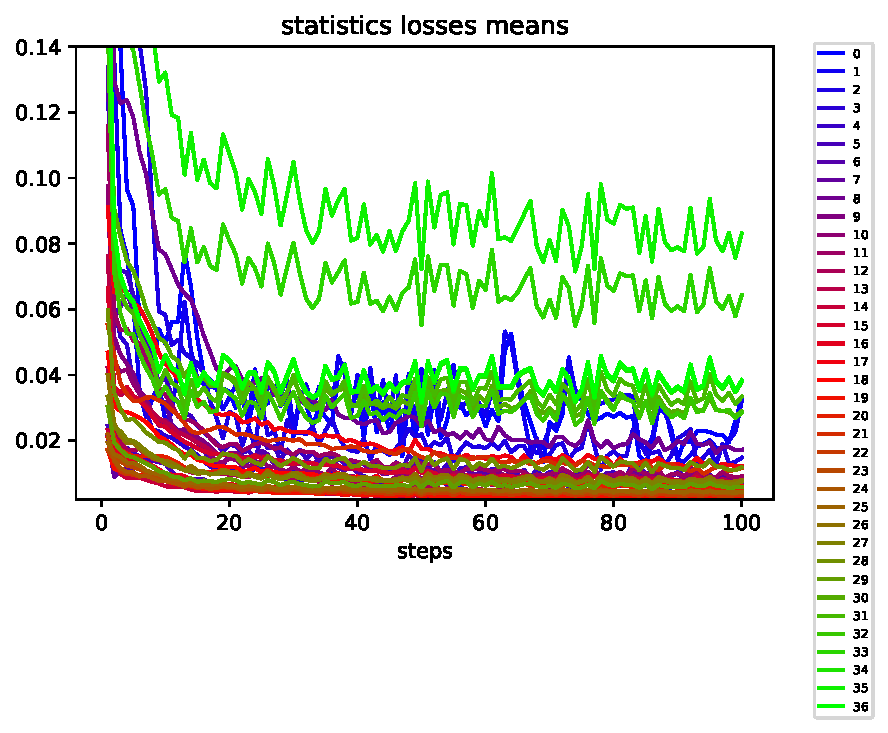
\includegraphics[
    width=\textwidth, 
    trim={0 0 1.6cm 0.6cm}, clip,
    ]{figures/reconstruction_CIFAR10_NN_ALL_metrics_statistics_losses_means.pdf}
    \end{minipage}%
    \begin{minipage}{0.45\textwidth}
    \centering
    \caption*{NN ALL CC}
    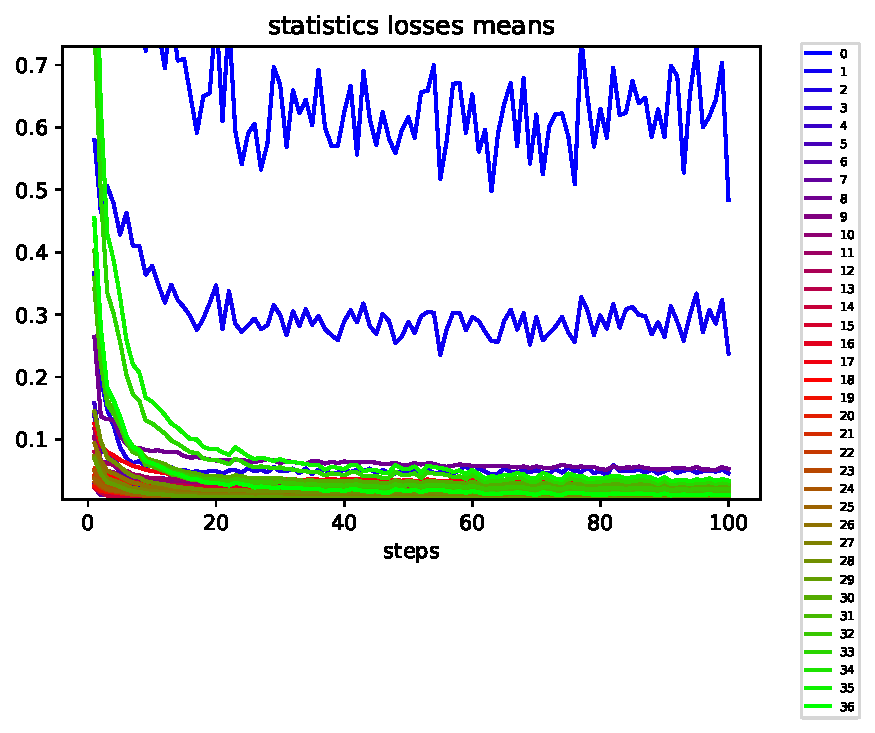
\includegraphics[
    width=\textwidth,
    trim={0 0 1.6cm 0.6cm}, clip,
    ]{figures/reconstruction_CIFAR10_NN_ALL_CC_metrics_statistics_losses_means.pdf}
    \end{minipage}
    \begin{minipage}{0.06\textwidth}
    \centering
    \vspace*{10pt}
    \setlength{\abovecaptionskip}{5pt plus 0pt minus 0pt}
    \setlength{\belowcaptionskip}{0pt plus 0pt minus 0pt}
    \caption*{\footnotesize Layer}
    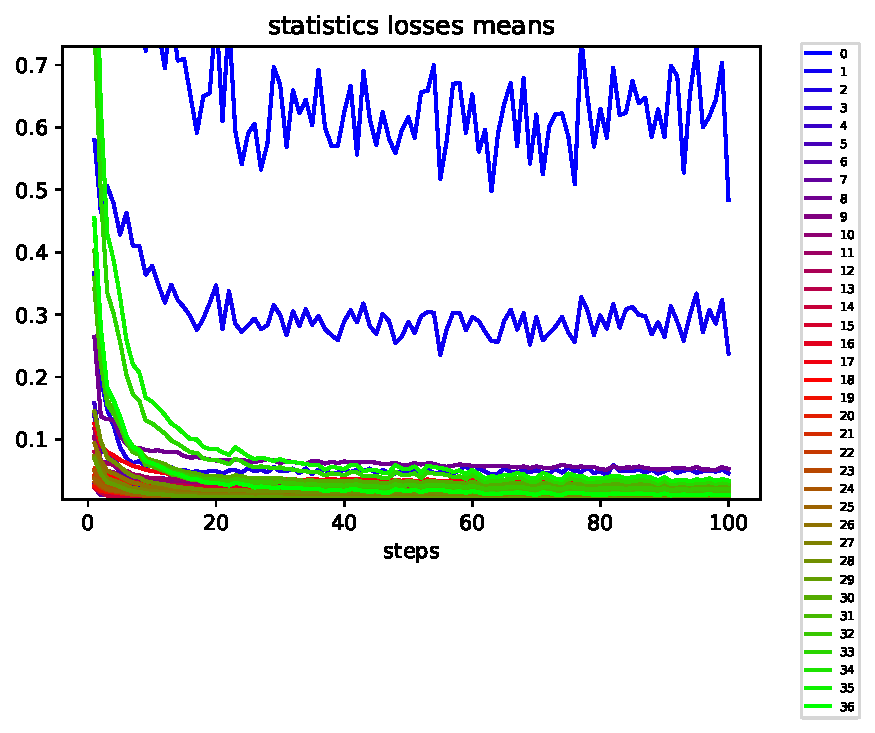
\includegraphics[
    width=\textwidth,
    trim={13.4cm 0 0 0.7cm}, clip,
    ]{figures/reconstruction_CIFAR10_NN_ALL_CC_metrics_statistics_losses_means.pdf}
    \end{minipage}
    }
    \caption{Loss coming from the difference in mean batch-statistics plotted per layer. 
    Lighter colors correspond to later layers in the network. \textit{Layer 0} is the input itself.}
    \label{fig:layer_losses}
\end{figure}

\begin{table}[!htbp]
\centering
\footnotesize
\pgfplotstabletypeset[
results,
images,
every row 1 column 1/.style={highlight},
every row 1 column 2/.style={highlight},
every row 1 column 3/.style={highlight},
every row 2 column 4/.style={highlight},
every row 1 column 5/.style={highlight},
every row 0 column 6/.style={highlight},
]{figures/unsupervised/reconstruction_CIFAR10_results.csv}
\caption{Metrics on reconstruction results in the unsupervised setting after 100 optimization epochs for CIFAR10}
\label{tab:cifar10results_unsupervised}
\end{table}

Finally, \cref{tab:cifar10results_unsupervised} presents results for the unsupervised setting.
Here, no label information is available and only the statistics-loss $r_\text{stats}$ is used.
Interestingly, these achieve better results than 
for the less complex GMM data set in an unsupervised setting (\cref{tab:gmm_results_raw}).
This leads one to conclude that the learned feature-representations of the neural network on
the CIFAR10 data set better capture invariances than those obtained for the GMM data set.


\subsection{Hyperparameter-Influence}


In the following, 
a grid search is performed on various hyperparameter settings 
to study their effect on the reconstruction outcome.
The search is performed on:
\begin{flalign*}
    s_\text{width} &\in \{4, 8, 16\} &\\
    s_\text{depth} &\in \{4, 8, 16\} \\
    n_{\set B} &\in \{128, 512, 1024, 2048\} \\
\end{flalign*}
For every hyperparameter setting ($s_\text{width}, s_\text{depth},  n_{\set B}$) 
of the Cartesian product of all possible values shown, a select number of metrics is reported.
The final outcome on the verification and validation accuracy for the method NN ALL CC is plotted in \cref{fig:rec_hyperparameter_search}.


\begin{figure}[!htbp]
\centering
    
    \caption*{\hspace*{6mm}NN ALL CC}
    \centerline{
    \hspace*{6mm}
    \begin{minipage}{0.6\textwidth}
    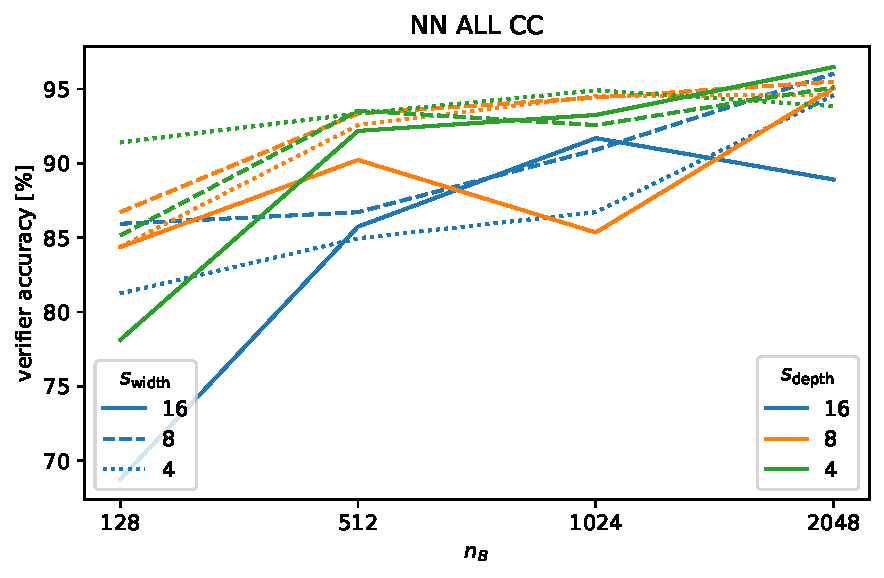
\includegraphics[
    trim={0 0 0 0.6cm}, clip,
    width=\textwidth
    ]{figures/comparison_CIFAR10_hyperparameters_verifier_accuracy_NN_ALL_CC.pdf}
    \end{minipage}%
    \begin{minipage}{0.6\textwidth}
    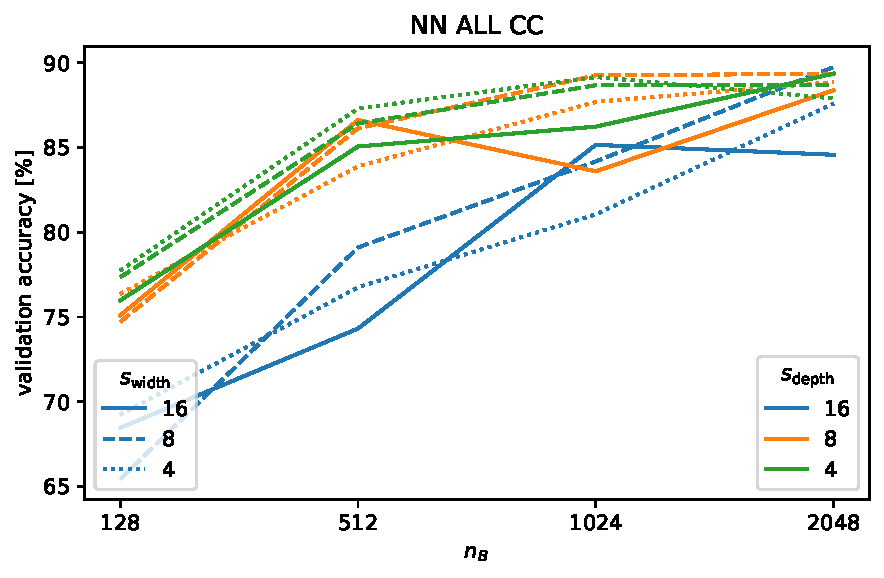
\includegraphics[
    trim={0 0 0 0.6cm}, clip,
    width=\textwidth
    ]{figures/comparison_CIFAR10_hyperparameters_validation_accuracy_NN_ALL_CC.pdf}
    \end{minipage}
    }
\caption{Reconstruction results for multiple hyperparameter settings on CIFAR10. 
Every data point depicts the end-results after 100 epochs.}
\label{fig:rec_hyperparameter_search}
\end{figure}


\begin{figure}[!htbp]
\centering
\caption*{NN ALL CC}
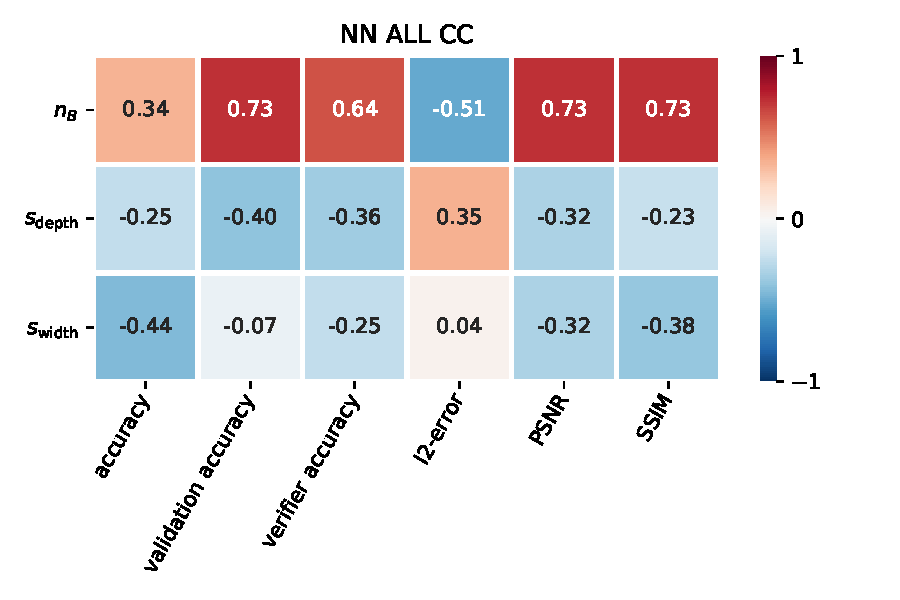
\includegraphics[
trim={0 0 0 0.75cm}, clip,
width=0.8\textwidth
]{figures/comparison_CIFAR10_hyperparameters_heatmap_NN_ALL_CC.pdf}
\caption{Hyperparameter correlation table}
\label{fig:rec_hyperparameter_heatmap}
\end{figure}

The positive influence of $n_{\set B}$ on the accuracy is quite clear, 
but the width and the depth of the reconstruction network is not. 
In fact, it seems as though an increase in complexity of the model is rather
detrimental to the scores.

The findings are solidified in \cref{fig:rec_hyperparameter_heatmap}, 
where a correlation heat map is given
between the parameters and the scores.

While $n_{\set B}$ is positively correlated for all scores 
(except for the l2-error, where a lower score is better), 
the other parameters show an almost inverse effect on what one would expect.
The larger reconstruction perform worse than simpler models 
However, these are likely to achieve higher scores after a longer training time. 

\subsection{Qualitative Results on Image Data Sets}
 

\begin{figure}[H]
{
    \centering
    
    \photostrip{\textit{Ground Truth}}{figures/reconstruction_MNIST_ground_truth.png}
    \photostrip{\textit{Distorted}}{figures/reconstruction_MNIST_distorted.png}
    \photostrip{CRITERION}{figures/reconstruction_MNIST_CRITERION_epoch_100.png}
    \photostrip{NN}{figures/reconstruction_MNIST_NN_epoch_100.png}
    \photostrip{NN CC}{figures/reconstruction_MNIST_NN_CC_epoch_100.png}
    \photostrip{NN ALL}{figures/reconstruction_MNIST_NN_ALL_epoch_100.png}
    \photostrip{NN ALL CC}{figures/reconstruction_MNIST_NN_ALL_CC_epoch_100.png}
}
\end{figure}
\begin{figure}[H]
    \centering
    
    \photostrip{RANDOM NN}{figures/reconstruction_MNIST_RANDOM_NN_epoch_100.png}
    \photostrip{RANDOM NN CC}{figures/reconstruction_MNIST_RANDOM_NN_CC_epoch_100.png}
    \photostrip{RP}{figures/reconstruction_MNIST_RP_epoch_100.png}
    \photostrip{RP CC}{figures/reconstruction_MNIST_RP_CC_epoch_100.png}
    \photostrip{RP ReLU}{figures/reconstruction_MNIST_RP_ReLU_epoch_100.png}
    \photostrip{RP ReLU CC}{figures/reconstruction_MNIST_RP_ReLU_CC_epoch_100.png}
    \photostrip{COMBINED CC}{figures/reconstruction_MNIST_COMBINED_CC_epoch_100.png}
    
    \caption{Results of the reconstruction task on MNIST data set after 100 epochs}
    \label{fig:MNIST_Images}
\end{figure}



% \subsubsection{CIFAR10}



\begin{figure}[H]
    \centering
    
    \photostrip{\textit{Ground Truth}}{figures/reconstruction_CIFAR10_ground_truth.png}
    \photostrip{\textit{Distorted}}{figures/reconstruction_CIFAR10_distorted.png}
    \photostrip{CRITERION}{figures/reconstruction_CIFAR10_CRITERION_epoch_100.png}
    \photostrip{NN}{figures/reconstruction_CIFAR10_NN_epoch_100.png}
    \photostrip{NN CC}{figures/reconstruction_CIFAR10_NN_CC_epoch_100.png}
    \photostrip{NN ALL}{figures/reconstruction_CIFAR10_NN_ALL_epoch_100.png}
    \photostrip{NN ALL CC}{figures/reconstruction_CIFAR10_NN_ALL_CC_epoch_100.png}
\end{figure}

\begin{figure}[H]
    \centering
    
    \photostrip{RANDOM NN}{figures/reconstruction_CIFAR10_RANDOM_NN_epoch_100.png}
    \photostrip{RANDOM NN CC}{figures/reconstruction_CIFAR10_RANDOM_NN_CC_epoch_100.png}
    \photostrip{RP}{figures/reconstruction_CIFAR10_RP_epoch_100.png}
    \photostrip{RP CC}{figures/reconstruction_CIFAR10_RP_CC_epoch_100.png}
    \photostrip{RP ReLU}{figures/reconstruction_CIFAR10_RP_ReLU_epoch_100.png}
    \photostrip{RP ReLU CC}{figures/reconstruction_CIFAR10_RP_ReLU_CC_epoch_100.png}
    \photostrip{COMBINED CC}{figures/reconstruction_CIFAR10_COMBINED_CC_epoch_100.png}
    
    \caption{Results of the reconstruction task on CIFAR10 data set after 100 epochs}
    \label{fig:CIFAR_Images}
\end{figure}

\begin{figure}[H]
    \centering
    
    \photostrip[5pt][16pt]{\textit{Ground Truth}}{figures/unsupervised/reconstruction_CIFAR10_ground_truth.png}
    \photostrip[5pt][16pt]{\textit{Distorted}}{figures/unsupervised/reconstruction_CIFAR10_distorted.png}
    \photostrip[5pt][16pt]{NN}{figures/unsupervised/reconstruction_CIFAR10_NN_epoch_100.png}
    \photostrip[5pt][16pt]{NN ALL}{figures/unsupervised/reconstruction_CIFAR10_NN_ALL_epoch_100.png}
    \photostrip[5pt][16pt]{RANDOM NN}{figures/unsupervised/reconstruction_CIFAR10_RANDOM_NN_epoch_100.png}
    \photostrip[5pt][16pt]{RP}{figures/unsupervised/reconstruction_CIFAR10_RP_epoch_100.png}
    
    \caption{Results of the reconstruction task on CIFAR10 data set in an unsupervised setting after 100 epochs}

    \label{fig:CIFAR_Images_unsupervised}
\end{figure}




\section{Inversion}




Although research in machine-learning is being made at a rapid pace,
the behavior and decision process of deep neural networks are 
still poorly understood and largely
regarded as black-box models.
The susceptibility of neural networks to adversarial attacks (\cite{moosavidezfooli2016deepfool}) has raised awareness
in security-critical areas (autonomous cars, ai in medical, face recognition).
This has sparked research need of explainable ai and interpretability.
Work unveiling the decision process of neural networks has been made 
(LRP (\cite{Bach2015OnPE}, Masking, Feature-Vis).
Feature-vis straightforward.. change input to maximally excite or minimize objective.
Receive examples of inputs.
Another concern raised by adversarial attacks has been regarding data privacy.
Sensitive patient data, personal information can be leaked.
Breaches in data privacy by adversarial attacks (\cite{carlini2020attack})
and attacks on data privacy algorithms (\cite{carlini2020extracting})


The following experiments have two goals.
One aims at better understanding the feature-representation of  
model by feature-visualization.
The other inspects what data of data set can be reconstructed by sharing statistics.


Danger of adversarial attacks has raised awareness for ai systems employed in 
security and safety sensitive areas.
Explainable Ai and interpretability have emerged as fields aiming to inspect the inner workings
of ai models to address robustness.
Lrp.. feature-visualisation.. exist. maximally excite neurons or optimize inputs for objective..
Along with adv attacks come data privacy concerns.. reconstruction gpt3, instahide, differential privacy.
Following experiments show results gaining insight into what optimal input for loss looks like..
Inspects what information is shared by statistics of layers..



\begin{figure}[H]
    \centering
    
    \photostrip[5pt]{CRITERION}{figures/inversion_MNIST_CRITERION_epoch_3000.png}
    \photostrip[5pt]{NN}{figures/inversion_MNIST_NN_epoch_3000.png}
    \photostrip[5pt]{NN CC}{figures/inversion_MNIST_NN_CC_epoch_3000.png}
    \photostrip[5pt]{NN ALL}{figures/inversion_MNIST_NN_ALL_epoch_3000.png}
    \photostrip[5pt]{NN ALL CC}{figures/inversion_MNIST_NN_ALL_CC_epoch_3000.png}
    \photostrip[5pt]{RANDOM NN}{figures/inversion_MNIST_RANDOM_NN_epoch_3000.png}
    \photostrip[5pt]{RANDOM NN CC}{figures/inversion_MNIST_RANDOM_NN_CC_epoch_3000.png}
\end{figure}

\begin{figure}[H]
    \centering
    
    \photostrip[5pt][20pt]{RP}{figures/inversion_MNIST_RP_epoch_3000.png}
    \photostrip[5pt][20pt]{RP CC}{figures/inversion_MNIST_RP_CC_epoch_3000.png}
    \photostrip[5pt][20pt]{RP ReLU}{figures/inversion_MNIST_RP_ReLU_epoch_3000.png}
    \photostrip[5pt][20pt]{RP ReLU CC}{figures/inversion_MNIST_RP_ReLU_CC_epoch_3000.png}
    \photostrip[5pt][20pt]{COMBINED CC}{figures/inversion_MNIST_COMBINED_CC_epoch_3000.png}
    
    \caption{Results of the inversion task on MNIST data set after 3000 epochs}
    \label{fig:MNIST_Images_Inversion}
\end{figure}



\begin{figure}[H]
    \centering
    
    \photostrip[5pt]{CRITERION}{figures/inversion_CIFAR10_CRITERION_epoch_3000.png}
    \photostrip[5pt]{NN}{figures/inversion_CIFAR10_NN_epoch_3000.png}
    \photostrip[5pt]{NN CC}{figures/inversion_CIFAR10_NN_CC_epoch_3000.png}
    \photostrip[5pt]{NN ALL}{figures/inversion_CIFAR10_NN_ALL_epoch_3000.png}
    \photostrip[5pt]{NN ALL CC}{figures/inversion_CIFAR10_NN_ALL_CC_epoch_3000.png}
    \photostrip[5pt]{RANDOM NN}{figures/inversion_CIFAR10_RANDOM_NN_epoch_3000.png}
    \photostrip[5pt]{RANDOM NN CC}{figures/inversion_CIFAR10_RANDOM_NN_CC_epoch_3000.png}
\end{figure}

\begin{figure}[H]
    \centering
    
    \photostrip[5pt][20pt]{RP}{figures/inversion_CIFAR10_RP_epoch_3000.png}
    \photostrip[5pt][20pt]{RP CC}{figures/inversion_CIFAR10_RP_CC_epoch_3000.png}
    \photostrip[5pt][20pt]{RP ReLU}{figures/inversion_CIFAR10_RP_ReLU_epoch_3000.png}
    \photostrip[5pt][20pt]{RP ReLU CC}{figures/inversion_CIFAR10_RP_ReLU_CC_epoch_3000.png}
    \photostrip[5pt][20pt]{COMBINED CC}{figures/inversion_CIFAR10_COMBINED_CC_epoch_3000.png}
    
    \caption{Results of the inversion task on CIFAR10 data set after 3000 epochs}
    \label{fig:CIFAR_Images_Inversion}
\end{figure}





\chapter{Conclusion}

In summary, it can be said that using the proposed loss formulations 
NN ALL and NN ALL CC can significantly 
aid in the reconstruction task.
While random projections might be 
well suited at capturing features 
of low-dimensional or comparatively simple data, 
they don't provide much practical use for complex image data sets.
Incorporating the non-linearity ReLU in the random projections (RP ReLU), in general, 
does not yield any notable differences in the performances.
This shows that the strength of the neural networks feature-representation
must come from the depth and hierarchical composition of convolutional feature extractors.
The increase in performance compared to a randomly initialized neural network
further shows that learned feature-representations are adapted to capture
important information about the data set.
The final effect of the class-conditional formulation is still to be verified.


MNIST <-> CIFAR 
CIFAR is forced to filter background noise.
The results show that...
neural networks are able to learn features that 
capture invariant properties of the data set.
By optimizing for image recognition, a lot of information
about the data set is implicitly stored in the shapes of their filters.
Also more explicitly, information about the data set is stored in the batchnorm layers
a lot of information in their layers
which can be used for dataset adaption and inverse tasks, such as deconvolution.













